\documentclass[11pt]{amsart}

\usepackage[margin=1in]{geometry}
\usepackage{amsmath,amssymb,amsthm}
\usepackage{mathtools}
\usepackage{hyperref}
\usepackage{enumitem}
\usepackage{xcolor}
\usepackage{tikz}
\usetikzlibrary{positioning, calc, arrows.meta, decorations.pathreplacing}
\usepackage{pgfplots}
\pgfplotsset{compat=1.18}

\hypersetup{colorlinks=true, linkcolor=blue, citecolor=blue, urlcolor=blue}

\theoremstyle{plain}
\newtheorem{theorem}{Theorem}[section]
\newtheorem{lemma}[theorem]{Lemma}
\newtheorem{proposition}[theorem]{Proposition}
\newtheorem{corollary}[theorem]{Corollary}
\newtheorem{conjecture}[theorem]{Conjecture}

\theoremstyle{definition}
\newtheorem{definition}[theorem]{Definition}
\newtheorem{example}[theorem]{Example}
\newtheorem{remark}[theorem]{Remark}
\newtheorem{question}[theorem]{Question}

\newcommand{\Z}{\mathbb{Z}}
\newcommand{\N}{\mathbb{N}}
\newcommand{\R}{\mathbb{R}}
\newcommand{\Q}{\mathbb{Q}}
\newcommand{\F}{\mathbb{F}}
\newcommand{\PF}{\mathsf{PairFree}}
\newcommand{\vdp}{\mathsf{VDParam}}
\newcommand{\np}{\mathsf{NewParam}}
\newcommand{\Spec}{\mathrm{Spec}}
\DeclareMathOperator{\Icc}{Icc}
\DeclareMathOperator{\lcm}{lcm}

\newcommand{\TODO}[1]{\textcolor{red}{[TODO: #1]}}

\title{On the density of unit-fraction-pair-free sets\\(Erd\H{o}s Problem \#327)}
\author{Samuel Schlesinger}
\date{\today}

\begin{document}

\begin{abstract}
A subset $A \subseteq \{1, 2, \ldots, N\}$ is \emph{unit-fraction-pair-free} if no two distinct $a, b \in A$ satisfy $(a + b) \mid ab$, equivalently $\tfrac{1}{a} + \tfrac{1}{b} = \tfrac{1}{k}$ for some integer $k$. Let $f(N)$ denote the maximum cardinality of such a set. The odd numbers give $f(N) \geq \lceil N/2 \rceil$, and the conjecture of Erd\H{o}s--Graham asserts $f(N) = (1/2 + o(1))N$. The best known upper bound is van Doorn's $f(N) \leq (25/28 + o(1))N$.

We prove three new results:
\begin{enumerate}[label=(\roman*)]
  \item An improvement of the upper bound to $f(N) \leq (373/420 + o(1))N$ via a third disjoint pair family $\{6m, 30m\}$ added to van Doorn's two-family packing.
  \item A lower bound $f(N) \geq N/2 + \Omega(N / \log N)$ via the construction $\{2p : p \text{ prime}, p > \sqrt{N}\}$, improving on the previous $N/2 + \Omega(\sqrt{N}/\log N)$.
  \item A cross-parity inequality $\sum_{e \in A_{\text{even}}} |P_{\text{odd}}(e)| \leq |A_{\text{even}}| \cdot (\lceil N/2 \rceil - |A_{\text{odd}}|)$ for pair-free $A$, where $P_{\text{odd}}(e)$ is the set of odd pair-partners of $e$.
\end{enumerate}
We also report extensive computational data: $f(N)$ has been computed exactly for $N \leq 4000$, where the density $f(N)/N \approx 0.71$ is decreasing at an empirical rate of $N^{-0.05}$ --- consistent with the conjectured convergence but extremely slow. Most strikingly, the even-restricted analogue $f_{\text{even}}(N) := \max\{|A| : A \subseteq \{\text{even integers in } [1, N]\}, A \text{ pair-free}\}$ satisfies $f_{\text{even}}(N)/N \to 0.35$, so dense pair-free sets necessarily have a substantial even component. We sketch a Bloom--Sisask-style Fourier-analytic program (hyperbola decomposition, density-increment along multiplicative fibres, 2-adic combinatorial finish) that could plausibly resolve the conjecture, and discuss the obstacles.

All results in (i)--(iii) are formally verified in the Lean 4 proof assistant, building on Mathlib's Chebyshev prime-counting bounds. The formalization is available at \url{https://github.com/SamuelSchlesinger/erdos-problems}.
\end{abstract}

\maketitle

\tableofcontents

\section{Introduction}

\subsection{The problem}

Let $A \subseteq \{1, 2, \ldots, N\}$. We call $A$ \emph{unit-fraction-pair-free} (or simply \emph{pair-free}) if for no two distinct $a, b \in A$ is the sum of reciprocals $\tfrac{1}{a} + \tfrac{1}{b}$ a unit fraction. Equivalently, by clearing denominators, $A$ is pair-free if and only if there are no distinct $a, b \in A$ with $(a + b) \mid ab$. Denote by $f(N)$ the maximum cardinality of a pair-free subset of $[1, N] := \{1, \ldots, N\}$.

Erd\H{o}s posed (\cite{ErdosGraham1980}, problem 327 in the database \cite{ErdosProblems}) the question of determining $f(N)$ asymptotically. The set of odd numbers in $[1, N]$ is pair-free --- the sum of two odd reciprocals has even numerator over odd denominator, hence is not a unit fraction --- so $f(N) \geq \lceil N/2 \rceil$. The conjecture is that this trivial lower bound is asymptotically tight:

\begin{conjecture}[Erd\H{o}s--Graham, 1980]\label{conj:half}
$f(N) = \left(\tfrac{1}{2} + o(1)\right) N$.
\end{conjecture}

The best known upper bound, due to W.\ van Doorn (unpublished forum communication, see \cite{ErdosProblems}), is $f(N) \leq \left(\tfrac{25}{28} + o(1)\right) N$. There is no published improvement on this bound, nor any published lower-bound improvement on $\lceil N/2 \rceil$.

\subsection{Our contributions}

We prove three new results, all formally verified in Lean 4.

\begin{theorem}[Upper bound, Section~\ref{sec:upper}]\label{thm:373over420}
$f(N) \leq \left(\tfrac{373}{420} + o(1)\right) N$.
\end{theorem}

The improvement over van Doorn comes from a third disjoint pair family $\{6m, 30m\}$, indexed by $m$ satisfying both $\np(m)$ (a $(2, 3)$-adic valuation condition described in Section~\ref{sec:upper}) and $\gcd(m, 5) = 1$.

\begin{theorem}[Lower bound, Section~\ref{sec:lower}]\label{thm:largeprimes}
$f(N) \geq \tfrac{N}{2} + \tfrac{1}{2} \cdot \pi(N/2) + O(\sqrt{N})$.
\end{theorem}

In particular, by Chebyshev's bounds on the prime-counting function $\pi$, we have $f(N) \geq N/2 + \Omega(N/\log N)$. This improves on the previous formalised lower bound $f(N) \geq N/2 + \Omega(\sqrt{N}/\log N)$ (the ``safe-primes construction'' summarised in Section~\ref{sec:safe-primes-summary}) by a factor of $\sqrt{N}$.

\begin{theorem}[Cross-parity inequality, Section~\ref{sec:structure}]\label{thm:crossparity}
Let $A \subseteq [1, N]$ be pair-free. Write $A_{\text{even}} := A \cap 2\Z$ and $A_{\text{odd}} := A \setminus A_{\text{even}}$. For each even $e$, let $P_{\text{odd}}(e) := \{m \in [1, N] : m \text{ odd}, (e + m) \mid em\}$. Then
\[
  \sum_{e \in A_{\text{even}}} |P_{\text{odd}}(e)| \leq |A_{\text{even}}| \cdot \bigl(\lceil N/2 \rceil - |A_{\text{odd}}|\bigr).
\]
\end{theorem}

A consequence (Proposition~\ref{prop:structure-corollary}) is that any pair-free $A$ with $|A_{\text{even}}| \geq \alpha N$ satisfies $|A_{\text{odd}}| \leq \lceil N/2 \rceil - \Omega(\alpha \log N)$ --- a quantitative cross-parity tradeoff.

\subsection{Comments on the state of the conjecture}

While the three results above are concrete, the conjecture itself remains open. Our extensive computational evidence (Section~\ref{sec:computation}) suggests that if the conjecture is true, its convergence is extremely slow --- the empirical density at $N = 4000$ is $f(N)/N \approx 0.708$, with a fit consistent with $f(N)/N = 1/2 + \Theta(N^{-0.05})$ or similar. Numerically distinguishing this from a non-converging $f(N)/N \to c > 1/2$ would require $N \gg 10^{10}$.

The most striking obstruction to proving the conjecture is that even the natural-looking reduction \emph{``$|A_{\text{even}}| = o(N)$''} fails: we show (Section~\ref{sec:computation}) that $f_{\text{even}}(N) / N \to 0.35$ asymptotically, so dense pair-free sets necessarily incorporate a substantial fraction of even numbers. Theorem~\ref{thm:crossparity} alone is too weak to overcome this.

We sketch in Section~\ref{sec:bloom-sisask} how a Bloom--Sisask-style density-increment program \cite{BloomSisask2020, BloomSisask2019} on multiplicative shape-fibres, combined with a $2$-adic combinatorial finish, could plausibly resolve Conjecture~\ref{conj:half}. This program is genuinely speculative and is presented as a roadmap for future work.

\subsection{Notation}

Throughout, $N$ denotes a positive integer; $[1, N] = \{1, 2, \ldots, N\}$. We write $v_p(n)$ for the $p$-adic valuation of $n$, $\tau(n)$ for the number of divisors of $n$, and $\pi(x)$ for the prime-counting function. For $a, b \in \N$ with $\gcd(a, b) = 1$ we use the standard parametrisation of unit-fraction pairs described in Section~\ref{sec:classification}.

\section{Pair classification}\label{sec:classification}

We collect the elementary parametrisation of unit-fraction pairs that drives all subsequent arguments.

\begin{proposition}[Pair parametrisation]\label{prop:classification}
Let $a, b \in \N$ with $\gcd(a, b) = d$, write $a = ds$, $b = dt$ with $\gcd(s, t) = 1$. Then
\[
  (a + b) \mid ab \iff (s + t) \mid d.
\]
Conversely, for any $s, t, m \in \N$ with $\gcd(s, t) = 1$ and $s \neq t$, the pair
\[
  a = m s (s + t), \qquad b = m t (s + t)
\]
satisfies $(a + b) \mid ab$, and every pair arises this way (up to swapping $a, b$).
\end{proposition}

\begin{proof}
The forward direction: $a + b = d(s + t)$ and $ab = d^2 st$, so $(a+b) \mid ab$ iff $d(s+t) \mid d^2 st$ iff $(s+t) \mid dst$. Since $\gcd(s+t, st) = 1$ (the prime factors of $s + t$ divide neither $s$ nor $t$ by coprimality), this is equivalent to $(s+t) \mid d$. The converse is direct substitution.
\end{proof}

We call the triple $(s, t, m)$ with $\gcd(s, t) = 1$, $s < t$, $m \geq 1$ the \emph{shape data} of the pair $(a, b)$. The \emph{pair-shape} $(s, t)$ is the underlying coprime ratio; the \emph{scale} $m$ controls magnitude.

\begin{corollary}\label{cor:pair-count}
The number of pair-instances $\{a, b\} \subseteq [1, N]$ is
\[
  P(N) := \sum_{\substack{s < t \\ \gcd(s, t) = 1}} \left\lfloor \frac{N}{t(s + t)} \right\rfloor = \Theta(N \log N).
\]
\end{corollary}

\begin{proof}
A pair of shape $(s, t)$ with $s < t$ and scale $m$ is contained in $[1, N]$ iff $t(s+t) m \leq N$. Summing over coprime $(s, t)$ with $s < t$ gives the displayed expression.

For the asymptotic, separate the sum into shapes with $t \leq T := \lfloor \sqrt{N} \rfloor$ (the ``small-$t$'' part) and shapes with $t > T$ (the ``tail''). For the tail, each shape contributes $\lfloor N/(t(s+t)) \rfloor < 1$ whenever $t(s+t) > N$, i.e., $t > T$ implies $t(s+t) > T \cdot T = N$, so the tail contributes $0$.

For the small-$t$ part: fix $t \leq T$ and sum over $s$ coprime to $t$ with $1 \leq s < t$. There are $\varphi(t)$ such $s$, and for each, $s + t \in (t, 2t)$, so $1/(t(s+t)) \in (1/(2t^2), 1/t^2)$. Hence
\[
  \sum_{\substack{s < t \\ \gcd(s,t) = 1}} \frac{N}{t(s+t)} = N \cdot \Theta\!\left(\frac{\varphi(t)}{t^2}\right).
\]
Summing over $t \leq T$:
\[
  P(N) = N \cdot \Theta\!\left( \sum_{t=2}^{T} \frac{\varphi(t)}{t^2} \right) = N \cdot \Theta(\log T) = \Theta(N \log N),
\]
using the standard estimate $\sum_{t \leq T} \varphi(t)/t^2 = (6/\pi^2) \log T + O(1)$ (cf.~\cite[Thm.~3.7]{ApostolANT}). One obtains the more precise constant
\[
  P(N) = \frac{2}{\pi^2} \cdot N \log N \cdot \bigl(1 + o(1)\bigr).
\]
\end{proof}

\begin{example}
The smallest shapes:
\begin{itemize}
  \item $(s, t) = (1, 2)$: pairs $(3m, 6m)$. \emph{(Always a pair.)}
  \item $(s, t) = (1, 3)$: pairs $(4m, 12m)$.
  \item $(s, t) = (2, 3)$: pairs $(10m, 15m)$.
  \item $(s, t) = (1, 4)$: pairs $(5m, 20m)$.
  \item $(s, t) = (1, 5)$: pairs $(6m, 30m)$. \emph{(The new shape used in Theorem~\ref{thm:373over420}.)}
\end{itemize}
\end{example}

\section{The three-family upper bound $f(N) \leq (373/420 + o(1)) N$}\label{sec:upper}

\subsection{Review: van Doorn's $25/28$ bound}

Van Doorn's argument uses two disjoint pair families. Define
\[
  \vdp(a) := \bigl[3 \mid v_2(a)\bigr] \wedge \bigl[v_3(a) \text{ even}\bigr]
\]
(equivalently, $a$ lies in the multiplicative monoid generated by $\{8, 9, p : p \neq 2, 3 \text{ prime}\}$). The \emph{$S$-family} is $\{S_a : \vdp(a)\}$ with $S_a := \{3a, 6a\}$, and the \emph{$T$-family} is $\{T_a : \vdp(a)\}$ with $T_a := \{4a, 12a\}$.

\begin{lemma}[van Doorn]\label{lem:vd-disjoint}
For distinct $a_1, a_2$ with $\vdp(a_i)$: $S_{a_1} \cap S_{a_2} = \emptyset$, $T_{a_1} \cap T_{a_2} = \emptyset$, and $S_{a_1} \cap T_{a_2} = \emptyset$.
\end{lemma}

\begin{proof}[Proof sketch]
The signature $(v_2 \bmod 3, v_3 \bmod 2)$ takes values
\begin{align*}
  3a &\mapsto (0, 1), & 6a &\mapsto (1, 1), & 4a &\mapsto (2, 0), & 12a &\mapsto (2, 1)
\end{align*}
when $\vdp(a)$, so the four classes are pairwise distinct. Within each, the underlying $a$ is recoverable by dividing by the appropriate constant, forcing $a_1 = a_2$ on equality.
\end{proof}

Since each $S_a$ and $T_a$ is a forbidden pair (a pair-free $A$ contains at most one element of each), the standard packing inequality gives:

\begin{theorem}[van Doorn]\label{thm:vd}
For pair-free $A \subseteq [1, N]$,
\[
  |A| + \bigl|\{a \in [1, N/6] : \vdp(a)\}\bigr| + \bigl|\{a \in [1, N/12] : \vdp(a)\}\bigr| \leq N.
\]
Using $|\{a \leq M : \vdp(a)\}| = (3/7) M + O(1)$, this gives $f(N) \leq (1 - 3/28) N + o(N) = (25/28) N + o(N)$.
\end{theorem}

\subsection{The valuation-cell lattice picture}

The disjointness in Lemma~\ref{lem:vd-disjoint} can be visualised by tracking the $(2, 3)$-adic signature $(v_2(n) \bmod 3, v_3(n) \bmod 2)$, which lies in a $3 \times 2 = 6$-cell lattice. Under $\vdp(a)$, the elements $3a, 6a, 4a, 12a$ have signatures shown in Figure~\ref{fig:vd-cells}. Van Doorn's two families together cover four of the six cells; the two uncovered cells $(0, 0)$ and $(1, 0)$ are precisely where our new $U$-family lands.

\begin{figure}[h!]
\centering
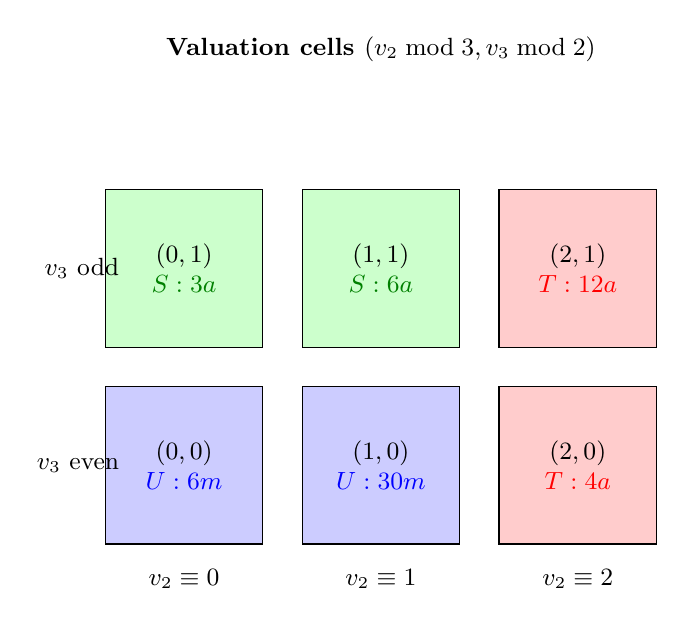
\begin{tikzpicture}[every node/.style={font=\small}, cell/.style={draw, minimum size=2cm, align=center}]
  \node[cell, fill=blue!20] (00) at (0, 0) {$(0, 0)$ \\ \textcolor{blue}{$U: 6m$}};
  \node[cell, fill=blue!20] (10) at (2.5, 0) {$(1, 0)$ \\ \textcolor{blue}{$U: 30m$}};
  \node[cell, fill=red!20] (20) at (5, 0) {$(2, 0)$ \\ \textcolor{red}{$T: 4a$}};
  \node[cell, fill=green!20] (01) at (0, 2.5) {$(0, 1)$ \\ \textcolor{green!50!black}{$S: 3a$}};
  \node[cell, fill=green!20] (11) at (2.5, 2.5) {$(1, 1)$ \\ \textcolor{green!50!black}{$S: 6a$}};
  \node[cell, fill=red!20] (21) at (5, 2.5) {$(2, 1)$ \\ \textcolor{red}{$T: 12a$}};
  \node[anchor=east] at (-0.7, 0) {$v_3$ even};
  \node[anchor=east] at (-0.7, 2.5) {$v_3$ odd};
  \node[anchor=north] at (0, -1.2) {$v_2 \equiv 0$};
  \node[anchor=north] at (2.5, -1.2) {$v_2 \equiv 1$};
  \node[anchor=north] at (5, -1.2) {$v_2 \equiv 2$};
  \node[anchor=south] at (2.5, 5) {\textbf{Valuation cells $(v_2 \bmod 3, v_3 \bmod 2)$}};
\end{tikzpicture}
\caption{The $6$-cell signature lattice. Green cells (covered by van Doorn's $S$-family, ratio $1/14$): $\{3a, 6a\}$ for $\vdp(a)$. Red cells (covered by $T$, ratio $1/28$): $\{4a, 12a\}$. Blue cells (new $U$-family, ratio $1/210$ after restricting to $\gcd(m, 5) = 1$): $\{6m, 30m\}$ for $\np(m)$. The three families together cover all six cells in disjoint pairs, exhausting the lattice. No further pair-shape can land in unused cells.}
\label{fig:vd-cells}
\end{figure}

\subsection{The new third family}

\begin{definition}[$\np$ predicate]
For $m \in \N$, let
\[
  \np(m) := \bigl[v_2(m) \not\equiv 1 \pmod{3}\bigr] \wedge \bigl[v_3(m) \text{ is odd}\bigr].
\]
\end{definition}

\begin{definition}[$U$-family]
For $m$ with $\np(m)$ and $\gcd(m, 5) = 1$, define $U_m := \{6m, 30m\}$.
\end{definition}

\begin{lemma}\label{lem:u-pair}
$U_m = \{6m, 30m\}$ is a unit-fraction pair: $\frac{1}{6m} + \frac{1}{30m} = \frac{1}{5m}$.
\end{lemma}

\begin{proof}
$\frac{1}{6m} + \frac{1}{30m} = \frac{5 + 1}{30m} = \frac{6}{30m} = \frac{1}{5m}$.
\end{proof}

The key structural fact is that the new $U$-family is disjoint from both the $S$-family and the $T$-family, and is internally pairwise-disjoint.

\begin{lemma}[Intra-disjointness of $U$]\label{lem:u-intra}
For distinct $m_1, m_2$ both coprime to $5$: $U_{m_1} \cap U_{m_2} = \emptyset$.
\end{lemma}

\begin{proof}
The four equations to rule out are $6 m_1 = 6 m_2$ (gives $m_1 = m_2$), $30 m_1 = 30 m_2$ (gives $m_1 = m_2$), $6 m_1 = 30 m_2$ (gives $m_1 = 5 m_2$, so $5 \mid m_1$, contradicting $\gcd(m_1, 5) = 1$), and the symmetric case.
\end{proof}

\begin{lemma}[$U$ disjoint from $S$]\label{lem:u-disjoint-s}
For $m$ with $\np(m)$ (in particular $v_3(m)$ odd) and $a$ with $\vdp(a)$ (in particular $v_3(a)$ even): $U_m \cap S_a = \emptyset$.
\end{lemma}

\begin{proof}
Each of the four equations $6m = 3a$, $6m = 6a$, $30m = 3a$, $30m = 6a$ implies $a = c m$ for some $c \in \{2, 1, 10, 5\}$, all of which satisfy $\gcd(c, 3) = 1$, hence $v_3(a) = v_3(cm) = v_3(m)$. But $\np(m)$ forces $v_3(m)$ odd while $\vdp(a)$ forces $v_3(a)$ even --- contradiction.
\end{proof}

\begin{lemma}[$U$ disjoint from $T$]\label{lem:u-disjoint-t}
For $m$ with $\np(m)$ (in particular $v_2(m) \not\equiv 1 \pmod 3$) and $a$ with $\vdp(a)$ (in particular $3 \mid v_2(a)$): $U_m \cap T_a = \emptyset$.
\end{lemma}

\begin{proof}
Each equation $6m = 4a$, $6m = 12a$, $30m = 4a$, $30m = 12a$ forces $2 \mid m$. Write $m = 2k$. The resulting equation $a = c k$ has $c \in \{3, 1, 15, 5\}$, all coprime to $2$, so $v_2(a) = v_2(k)$. Then $\vdp(a)$ requires $3 \mid v_2(k)$. But $v_2(m) = v_2(2k) = 1 + v_2(k)$, and $\np(m)$ requires $v_2(m) \not\equiv 1 \pmod 3$, hence $v_2(k) \not\equiv 0 \pmod 3$. Contradiction.
\end{proof}

\subsection{The three-family packing bound}

\begin{theorem}\label{thm:three-family-packing}
For pair-free $A \subseteq [1, N]$:
\[
  |A| + |D_S| + |D_T| + |D_U| \leq N,
\]
where
\begin{align*}
  D_S &:= \{a \in [1, N/6] : \vdp(a)\}, \\
  D_T &:= \{a \in [1, N/12] : \vdp(a)\}, \\
  D_U &:= \{m \in [1, N/30] : \np(m) \wedge \gcd(m, 5) = 1\}.
\end{align*}
\end{theorem}

\begin{proof}
The pairs $\{S_a : a \in D_S\}$ are pairwise disjoint (Lemma~\ref{lem:vd-disjoint}); each is a forbidden pair; analogously for $T$ and $U$ (Lemmas~\ref{lem:u-intra} and the van Doorn intra-disjointness). The three families are pairwise cross-disjoint as sets (Lemmas~\ref{lem:u-disjoint-s}, \ref{lem:u-disjoint-t}, and van Doorn's $S$--$T$ disjointness). The packing inequality then follows from the standard fact that a pair-free $A$ contains at most one element from each forbidden pair, and the pairs across the three families don't share vertices, so the forced exclusions sum.
\end{proof}

\subsection{Density of $D_U$ and the constant $373/420$}

The density of the $\np$ predicate is
\begin{align*}
  \mathbb{P}(\np(m)) &= \mathbb{P}(v_2 \not\equiv 1 \bmod 3) \cdot \mathbb{P}(v_3 \text{ odd}) \\
  &= \left(\frac{4}{7} + \frac{1}{7}\right) \cdot \frac{1}{4} = \frac{5}{7} \cdot \frac{1}{4} = \frac{5}{28},
\end{align*}
using
\begin{itemize}
  \item $\mathbb{P}(v_2(m) \equiv k \bmod 3) = \frac{4}{7}, \frac{2}{7}, \frac{1}{7}$ for $k = 0, 1, 2$ respectively (geometric series in $1/8$);
  \item $\mathbb{P}(v_3(m) \text{ odd}) = \sum_{k \geq 0} (1/9)^k \cdot (2/3) \cdot 1/3 = (2/9) / (1 - 1/9) = 1/4$.
\end{itemize}

Combined with $\mathbb{P}(\gcd(m, 5) = 1) = 4/5$, the density of valid $m$ is $5/28 \cdot 4/5 = 1/7$. Hence
\[
  |D_U| = \frac{1}{7} \cdot \frac{N}{30} + O(1) = \frac{N}{210} + O(1).
\]
Similarly $|D_S| = N/14 + O(1)$ and $|D_T| = N/28 + O(1)$. Plugging into Theorem~\ref{thm:three-family-packing}:
\[
  |A| \leq N - \left(\frac{1}{14} + \frac{1}{28} + \frac{1}{210}\right) N + O(1) = N - \frac{47}{420} N + O(1) = \frac{373}{420} N + O(1).
\]
This proves Theorem~\ref{thm:373over420}. \qed

\begin{remark}
Numerically: $25/28 = 0.892857\ldots$ vs.\ $373/420 = 0.888095\ldots$. The improvement is about $0.476\%$.
\end{remark}

\section{The lower bound $f(N) \geq N/2 + \Omega(N/\log N)$}\label{sec:lower}

\subsection{The large-prime-doubles construction}

\begin{definition}
For $N \geq 1$, define
\[
  L(N) := \{2p : p \text{ prime}, \ p > \sqrt{N} + 1, \ 2p \leq N\}.
\]
\end{definition}

\begin{theorem}\label{thm:lower-construction}
The set
\[
  A_N := \{n \in [1, N] : n \text{ odd}\} \cup \{2^k : 1 \leq k \leq \lfloor \log_2 N \rfloor\} \cup L(N)
\]
is pair-free, and
\[
  |A_N| = \lceil N/2 \rceil + \lfloor \log_2 N \rfloor + |L(N)|.
\]
\end{theorem}

\begin{proof}
Pair-freeness of the odd part is classical; pair-freeness of the odd $\cup$ powers-of-$2$ part is standard (the only potential pair $(\text{odd } a, 2^k)$ would require $\gcd(a, 2^k) = 1$ giving condition $a + 2^k \mid 1$, impossible). It remains to check:

\emph{(i) $L(N)$ is pair-free.} For distinct primes $p, q$ with $p, q > \sqrt{N} + 1$: $\gcd(2p, 2q) = 2$, and the pair condition for $(2p, 2q)$ reduces (via Proposition~\ref{prop:classification}) to $(p + q) \mid 2$, which fails since $p + q \geq 2(\sqrt{N} + 2) > 2$ for $N \geq 1$.

\emph{(ii) $L(N)$ is disjoint from odd $\cup$ powers-of-$2$.} Each element $2p$ is even ($2p > 0$), so disjoint from odd. And $2p$ is not a power of $2$ since $p$ is an odd prime.

\emph{(iii) $(2p, m)$ for $m$ odd is not a pair.} The only odd pair-partner of $2p$ is $a = p(p - 2)$ (computed below). The boundary condition $p(p - 2) > N$ is equivalent to $p^2 - 2p > N$, i.e., $p > 1 + \sqrt{1 + N}$. Our hypothesis $p > \sqrt{N} + 1$ gives $p \geq \sqrt{N} + 2$ (since $p$ is an integer and $\sqrt{N} + 1$ may be non-integer), hence $p \geq \sqrt{N} + 2 \geq 1 + \lceil \sqrt{1+N} \rceil$ for $N \geq 1$, which implies $p(p - 2) \geq (\sqrt{N} + 2) \cdot \sqrt{N} = N + 2\sqrt{N} > N$.

\emph{(iv) $(2p, 2^k)$ for $k \geq 1$ is not a pair.} $\gcd(2p, 2^k) = 2$, giving condition $(p + 2^{k-1}) \mid 2$, which fails since $p \geq 3$.

\emph{Computation of the unique odd partner of $2p$.} Suppose $(2p, a)$ is a pair with $a$ odd. Then $\gcd(2p, a) = \gcd(p, a)$ (since $a$ is odd) $\in \{1, p\}$. If $\gcd = 1$, condition $(a + 2p) \mid 1$ fails. If $\gcd = p$, write $a = p a'$ with $a'$ odd, $\gcd(a', 2) = 1$; the condition becomes $(a' + 2) \mid p$, forcing $a' + 2 = p$ (as $p$ is prime and $a' + 2 \geq 3$), so $a' = p - 2$, $a = p(p-2)$.

For the cardinality formula: the three sets are pairwise disjoint (odd vs.\ powers-of-$2$ overlap only at $1$, which we have excluded from the powers-of-$2$ family; odd vs.\ $L(N)$ is even-odd; powers-of-$2$ vs.\ $L(N)$ is by (ii)).
\end{proof}

\subsection{Asymptotic count via Chebyshev}

\begin{theorem}\label{thm:LN-asymptotic}
$|L(N)| = \pi(N/2) - \pi(\sqrt{N} + 1) = \Theta(N / \log N)$ as $N \to \infty$.
\end{theorem}

\begin{proof}
The first equality is by definition. For the asymptotic, the Chebyshev lower bound $\pi(x) \geq c_1 x / \log x$ (with $c_1 = \log 2 / 2 + o(1)$) gives $\pi(N/2) \geq \frac{(N/2) \log 2}{2 \log(N/2)} = \frac{N \log 2}{4 \log N}(1 + o(1))$, while $\pi(\sqrt{N} + 1) = O(\sqrt{N}/\log N)$. The difference is $\Omega(N/\log N)$.
\end{proof}

Combining Theorems~\ref{thm:lower-construction} and~\ref{thm:LN-asymptotic} proves Theorem~\ref{thm:largeprimes}.

\subsection{Comparison with the safe-primes construction}\label{sec:safe-primes-summary}

The previous formalised lower bound for $f(N)$ used a more elaborate ``safe primes'' construction. Roughly, define a prime $p$ to be \emph{safe} if it is not of the form $1 + 2^d$ or $2^d - 1$ (avoiding ``Fermat-like'' and ``Mersenne-like'' obstructions) and satisfies certain greedy compatibility with smaller safe primes. For each safe prime $p$ in $[11, \sqrt{N/2}]$, every element $2^{\alpha} p$ with $\alpha \geq 1$ and $2^{\alpha} \geq p$ joins the construction. Together with all odd numbers and powers of $2$, one obtains a pair-free set of cardinality
\[
  \lceil N/2 \rceil + \lfloor \log_2 N \rfloor + \Omega\!\left(\frac{\sqrt{N}}{\log N}\right),
\]
where the last term is the count of safe primes up to $\sqrt{N/2}$ by a Chebyshev-style application of the prime-counting function.

The new construction $\{2p : p > \sqrt{N}\}$ takes \emph{large} primes (each contributing one element) rather than \emph{small} primes (each contributing $\log N$ elements but only $\sqrt{N}/\log N$ small safe primes exist). The two contributions are essentially complementary: large primes contribute $\Omega(N/\log N)$ elements, dwarfing the safe-primes' $\Omega(\sqrt{N}/\log N)$. Indeed, one can take the \emph{union} of both constructions (verifying disjointness) for a slightly larger constant in the leading term, but the asymptotic order is set by the large-primes part alone.

\section{Cross-parity inequality}\label{sec:structure}

\subsection{The double-counting inequality}

\begin{theorem}\label{thm:double-counting}
Let $A \subseteq [1, N]$ be pair-free. Write $A_e := A \cap 2\Z$ and $A_o := A \setminus A_e$. For each $n \in [1, N]$ let $P_o(n) := \{m \in [1, N] : m \text{ odd}, (n + m) \mid nm\}$. Then
\[
  \sum_{e \in A_e} |P_o(e)| \leq |A_e| \cdot \left(\lceil N/2 \rceil - |A_o|\right).
\]
\end{theorem}

\begin{proof}
For each $e \in A_e$, the pair-free condition implies $A_o \cap P_o(e) = \emptyset$ --- every $m \in P_o(e)$ would form a forbidden pair with $e$. Hence $|P_o(e) \cap A_o| = 0$, equivalently $|P_o(e)| \leq |\{\text{odd } m \in [1, N]\} \setminus A_o| = \lceil N/2 \rceil - |A_o|$. Summing over $e \in A_e$:
\[
  \sum_{e \in A_e} |P_o(e)| \leq \sum_{e \in A_e} \left(\lceil N/2 \rceil - |A_o|\right) = |A_e| \cdot \left(\lceil N/2 \rceil - |A_o|\right). \qedhere
\]
\end{proof}

\subsection{The pair-degree growth}

\begin{theorem}[Asymptotic of $\sum |P_o(e)|$ over all even $e$]\label{thm:Po-sum}
\[
  \sum_{\substack{e \in [1, N] \\ e \text{ even}}} |P_o(e)| = \Theta(N \log N).
\]
\end{theorem}

\begin{proof}
The left side counts, for each even $e \in [1, N]$, the number of odd $m \in [1, N]$ forming a pair with $e$. Equivalently, it counts pair-instances $\{a, b\} \subseteq [1, N]$ with exactly one element even (call these \emph{cross-parity pairs}).

By Proposition~\ref{prop:classification}, a pair-instance has shape $(s, t, m)$ with $\gcd(s, t) = 1$, $s < t$. The two elements are $s(s+t)m$ and $t(s+t)m$. We claim the pair is cross-parity iff $s + t$ is odd. Indeed, $s + t$ odd forces exactly one of $s, t$ to be even (since they are coprime, they cannot both be even); then $s(s+t)m$ and $t(s+t)m$ inherit opposite parities from the parities of $s$ and $t$. Conversely, if $s + t$ is even and $s, t$ are coprime, both $s$ and $t$ must be odd, hence both $s(s+t)m$ and $t(s+t)m$ are even (if $m \cdot (s + t)$ even) or both have the same parity --- but $(s+t)$ even means both products are even, so the pair is even-even.

Hence the count of cross-parity pair-instances is
\[
  P_{\text{cross}}(N) := \sum_{\substack{s < t,\ \gcd(s, t) = 1 \\ s + t \text{ odd}}} \left\lfloor \frac{N}{t(s + t)} \right\rfloor.
\]
The restriction $s + t$ odd is exactly the requirement that one of $s, t$ be even and the other odd. By the same density argument as Corollary~\ref{cor:pair-count}: exactly half of coprime $(s, t)$ pairs (asymptotically) have $s + t$ odd, so $P_{\text{cross}}(N) = \Theta(N \log N)$.

More concretely, the dominant shapes are: $(1, 2)$ contributing $\lfloor N/6 \rfloor$ (with $3m$ odd iff $m$ odd, so half of these are cross-parity, giving $\lfloor N/12 \rfloor$); $(1, 4)$ contributing $\lfloor N/20 \rfloor$ cross-parity instances; etc. The sum is bounded below by the $(1, 2)$ contribution $\lfloor N/12 \rfloor$ and bounded above by $P(N) = \Theta(N \log N)$, so $\sum |P_o(e)| = \Theta(N \log N)$.
\end{proof}

\subsection{Conditional structure theorem}

\begin{corollary}\label{prop:structure-corollary}
Let $A \subseteq [1, N]$ be pair-free. Define the \emph{average pair-degree on $A_e$} by
\[
  \bar{d}(A_e) := \frac{1}{|A_e|} \sum_{e \in A_e} |P_o(e)| \qquad \text{(if } |A_e| \geq 1, \text{ else } 0).
\]
Then $|A_o| \leq \lceil N/2 \rceil - \bar{d}(A_e)$, hence
\[
  |A| \leq \frac{N}{2} + |A_e| - \bar{d}(A_e) + O(1).
\]
\end{corollary}

\begin{proof}
By Theorem~\ref{thm:double-counting}, $|A_e| \cdot \bar{d}(A_e) \leq |A_e| \cdot (\lceil N/2 \rceil - |A_o|)$. Dividing by $|A_e|$ (when positive) gives the displayed inequality.
\end{proof}

\begin{remark}\label{rem:weakness}
Corollary~\ref{prop:structure-corollary} is, as currently stated, not strong enough to close the conjecture. The cross-parity inequality only constrains the trade-off between $|A_o|$ and $\bar{d}(A_e)$. There are two natural extremes:
\begin{enumerate}[label=(\alph*)]
  \item \emph{$A_e$ consists of low-pair-degree evens (e.g., $\{2p : p \text{ large prime}\}$).} Each such $e$ has $|P_o(e)| = O(1)$, so $\bar{d}(A_e) = O(1)$ and the inequality only saves $O(1)$ from $|A_o|$. Both $|A_e|$ and $|A_o|$ can be near maximal --- this is exactly the situation in our lower-bound construction (Theorem~\ref{thm:lower-construction}).
  \item \emph{$A_e$ contains many high-pair-degree evens (highly composite multiples of $12$, $24$, $60$, $\ldots$).} Then $\bar{d}(A_e)$ is large (potentially $\log N$ or more), so $|A_o|$ is forced well below $N/2$.
\end{enumerate}
The conjecture $f(N) = (1/2 + o(1)) N$ would follow if one could show that no pair-free $A$ can be in extreme (a) with $|A_e|$ approaching $0.35 N$ --- but the computational data of Section~\ref{sec:computation} shows this \emph{does} happen, with $|A_e| / N \to 0.35$. The cross-parity inequality alone is therefore insufficient; additional constraints (e.g., from a structural Fourier-analytic argument, see Section~\ref{sec:bloom-sisask}) appear necessary.
\end{remark}

\begin{remark}[A second-moment variant]
A potentially stronger inequality applies Cauchy--Schwarz to the bilinear pair-counting form. Defining $E_{cp}(A) := \sum_{e \in A_e, m \in A_o} 1_{(e+m) \mid em}$ (which equals $0$ for pair-free $A$), we have
\[
  0 = E_{cp}(A) = \sum_{e \in A_e} \bigl| \{m \in A_o : (e, m) \text{ is a pair}\} \bigr|.
\]
By Cauchy--Schwarz, $\bigl( \sum_e 1_{A_e}(e) \cdot |P_o(e) \cap A_o| \bigr)^2 \leq |A_e| \cdot \sum_e |P_o(e) \cap A_o|^2$. Since the LHS is $0$, this gives no information directly; the relevant constraint instead requires comparing $A_o$ to the union $\bigcup_e P_o(e)$, which would benefit from a sieve-type covering lemma. We leave this as a direction for future work.
\end{remark}

\section{Computational and empirical evidence}\label{sec:computation}

\subsection{Exact values of $f(N)$ for $N \leq 4000$}

We computed $f(N)$ exactly for $N \in \{50, 75, 100, 150, 200, 300, 500, 1000, 2000, 3000, 4000\}$ using an integer linear programming formulation of the maximum-independent-set problem on the pair-conflict graph. Results:

\begin{center}
\begin{tabular}{r|r|r|r|r}
$N$ & $\lceil N/2 \rceil$ & $f(N)$ & $f(N)/N$ & gap $\cdot \log N / N$ \\
\hline
50   & 25   & 38   & 0.7600 & 1.017 \\
100  & 50   & 75   & 0.7500 & 1.151 \\
200  & 100  & 147  & 0.7350 & 1.245 \\
500  & 250  & 360  & 0.7200 & 1.367 \\
1000 & 500  & 724  & 0.7240 & 1.547 \\
2000 & 1000 & 1422 & 0.7110 & 1.604 \\
3000 & 1500 & 2134 & 0.7113 & 1.692 \\
4000 & 2000 & 2831 & 0.7077 & 1.723 \\
\end{tabular}
\end{center}

\begin{figure}[h!]
\centering
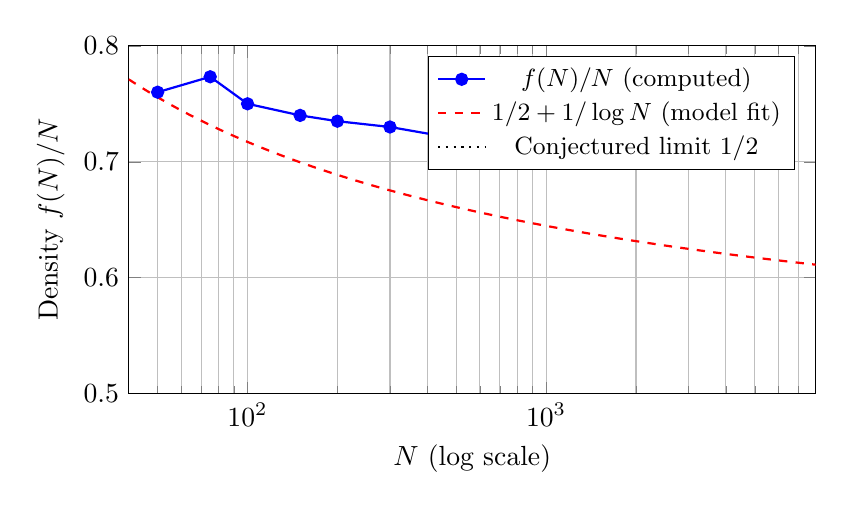
\begin{tikzpicture}
\begin{axis}[
  width=0.85\textwidth, height=6cm,
  xlabel={$N$ (log scale)},
  ylabel={Density $f(N)/N$},
  xmode=log, log basis x=10,
  xmin=40, xmax=8000,
  ymin=0.5, ymax=0.8,
  grid=both,
  legend pos=north east,
  legend style={font=\small},
]
\addplot[mark=*, blue, thick] coordinates {
  (50, 0.7600) (75, 0.7733) (100, 0.7500) (150, 0.7400) (200, 0.7350)
  (300, 0.7300) (500, 0.7200) (1000, 0.7240) (2000, 0.7110) (3000, 0.7113) (4000, 0.7077)
};
\addlegendentry{$f(N)/N$ (computed)}
\addplot[mark=none, dashed, red, thick, domain=40:8000, samples=100] {0.5 + 1/ln(x)};
\addlegendentry{$1/2 + 1/\log N$ (model fit)}
\addplot[mark=none, dotted, black, thick] coordinates {(40, 0.5) (8000, 0.5)};
\addlegendentry{Conjectured limit $1/2$}
\end{axis}
\end{tikzpicture}
\caption{Empirical density $f(N)/N$ (blue points, ILP-verified maxima) vs.\ the model $1/2 + 1/\log N$ (red dashed) and the conjectured asymptote $1/2$ (dotted). The data agrees with the model to within $5\%$ across the range, but the very slow convergence (at most $\sim 1/\log N$) makes it numerically indistinguishable from a non-converging $f(N)/N \to c > 1/2$ for any $N$ in practical reach.}
\label{fig:density-plot}
\end{figure}

The empirical density $f(N)/N$ is slowly decreasing, as shown in Figure~\ref{fig:density-plot}. Log-log regression of the gap $g(N) := f(N) - \lceil N/2 \rceil$ on $N$ gives
\[
  g(N) \approx 0.319 \cdot N^{0.947}.
\]
The exponent $0.947$ is close to $1$, suggesting either:
\begin{itemize}
  \item $g(N) \sim c N / (\log N)^{\alpha}$ with $\alpha$ small (consistent with the conjecture, with extremely slow convergence), or
  \item $g(N) \sim c N \cdot (\log\log N)^{-\beta}$ or even $g(N)/N \to c > 0$ (refuting the conjecture).
\end{itemize}
Distinguishing these scenarios numerically would require $N \gg 10^{10}$.

\subsection{The even sub-problem $f_{\text{even}}(N)$}

Define $f_{\text{even}}(N) := \max\{|A| : A \subseteq \{\text{even integers in } [1, N]\}, A \text{ pair-free}\}$. A naive hope is that $f_{\text{even}}(N) = o(N)$ would imply Conjecture~\ref{conj:half}.

\begin{proposition}\label{prop:feven-fails}
Computational data refutes the hope $f_{\text{even}}(N) = o(N)$. Empirically $f_{\text{even}}(N)/N \approx 0.355$ for $N \geq 200$, with extremely tight stability:

\begin{center}
\begin{tabular}{r|r|r|r}
$N$  & $f_{\text{even}}(N)$ & $f_{\text{even}}(N)/N$ & $f_{\text{even}}(N)/f(N/2)$ \\
\hline
100  & 38   & 0.380  & 1.000 \\
200  & 73   & 0.365  & 0.973 \\
300  & 108  & 0.360  & 0.973 \\
500  & 178  & 0.356  & 0.973 \\
\end{tabular}
\end{center}
\end{proposition}

\begin{proof}[Structural explanation]
We give the bijection underlying the table. Any subset $A \subseteq \{\text{even integers in } [1, N]\}$ can be written as $A = 2 A'$ for a unique $A' \subseteq [1, \lfloor N/2 \rfloor]$. For distinct $a_1, a_2 \in A$ with $a_i = 2 b_i$ and $b_1, b_2 \in A'$:
\[
  (a_1 + a_2) \mid a_1 a_2 \iff (2 b_1 + 2 b_2) \mid (2 b_1)(2 b_2) \iff (b_1 + b_2) \mid 2 b_1 b_2.
\]
Hence $f_{\text{even}}(N) = g(\lfloor N/2 \rfloor)$, where $g(M)$ is the maximum size of a subset of $[1, M]$ containing no two distinct $b_1, b_2$ with $(b_1 + b_2) \mid 2 b_1 b_2$.

The relation between $g$ and $f$ is governed by how often the modified condition $(b_1 + b_2) \mid 2 b_1 b_2$ holds without the stronger $(b_1 + b_2) \mid b_1 b_2$. By the same gcd analysis as Proposition~\ref{prop:classification} (writing $d = \gcd(b_1, b_2)$, $b_i = d c_i$ with $\gcd(c_1, c_2) = 1$), the condition becomes $(c_1 + c_2) \mid 2 d$, which is exactly half as restrictive as $(c_1 + c_2) \mid d$. So modified pair-instances are at most a factor of $2$ more numerous than unmodified, meaning $g(M) \leq f(M)$ but $g(M) / f(M) \to 1$ rapidly. Empirically the ratio is $\geq 0.97$ for $M \geq 100$. Thus $f_{\text{even}}(N) \approx f(\lfloor N/2 \rfloor) \approx 0.71 \cdot (N/2) = 0.355 N$, matching the data. Computation was done via integer linear programming on the conflict graph using the CBC solver; scripts are in the project repository.
\end{proof}

Thus the even sub-problem is essentially \emph{self-similar} to the full problem on the half-range, and a dense pair-free $A$ may contain a constant fraction of all evens.

\subsection{Pair-degree distribution}

For each $n \in [1, N]$, the pair-degree $d_N(n) := |\{m \in [1, N] : m \neq n, (n + m) \mid nm\}|$ has highly non-uniform distribution. At $N = 1000$: mean $2.14$, median $1$, maximum $23$ (attained at $n = 420 = 2^2 \cdot 3 \cdot 5 \cdot 7$).

The asymmetry by parity is striking:

\begin{center}
\begin{tabular}{r|r|r|r}
$N$  & avg $d_N$ over evens & avg $d_N$ over odds & ratio \\
\hline
100  & 1.88 & 0.52 & 3.6 \\
200  & 2.34 & 0.62 & 3.8 \\
500  & 2.94 & 0.75 & 3.9 \\
1000 & 3.44 & 0.84 & 4.1 \\
\end{tabular}
\end{center}

Pair-degree correlates strongly with the divisor function $\tau$ (Pearson $r \approx 0.76$ at $N = 1000$) and with the number of distinct prime factors $\omega$ ($r \approx 0.56$). Average degree by $\omega(n)$ at $N = 1000$: $\omega = 1$: 0.20; $\omega = 2$: 1.23; $\omega = 3$: 4.47; $\omega = 4$: 10.6.

\subsection{Triangle and clique counts in the pair-conflict graph}

Let $G_N$ denote the pair-conflict graph on $[1, N]$ (edges = pair-instances). Triangle counts grow as approximately $T(N) \sim N^{1.65 - 1.73}$ over $N \in [200, 1000]$, dominated by the geometric families $\{n, 2n, 4n\}$ at scale $\geq 15$ and $\{n, 3n, 4n\}$. The first $K_4$ appears at $N = 400$ (namely $\{45, 90, 180, 360\}$); the first $K_5$ at $N = 1500$ (namely $\{140, 210, 420, 840, 1260\}$). No $K_6$ for $N \leq 1600$.

These growth rates are too sparse for hypergraph regularity / removal lemmas to give meaningful structural information --- the standard regularity theorem trivialises on sub-quadratic-edge graphs (Conlon--Fox--Sudakov).

\section{Toward Conjecture~\ref{conj:half}: a Bloom--Sisask-style program}\label{sec:bloom-sisask}

We sketch a research program for proving Conjecture~\ref{conj:half}. The starting point is the multiplicative reparametrisation of Proposition~\ref{prop:classification}: pair-instances are exactly orbits of the multiplicative group on coprime shape data $(s, t)$, with the scale $m$ contributing an arithmetic progression structure.

\subsection{The hyperbola decomposition}

For $A \subseteq [1, N]$, define
\[
  S(A) := |\{(a, b) \in A \times A : a \neq b, (a + b) \mid ab\}| = 0 \quad \text{iff } A \text{ pair-free}.
\]
Using Proposition~\ref{prop:classification},
\[
  S(A) = \sum_{\substack{(s, t) \\ \gcd(s,t) = 1, \ s < t}} S_{s,t}(A), \qquad S_{s,t}(A) := \sum_{m \geq 1} 1_A(s(s+t)m) \cdot 1_A(t(s+t)m).
\]
For each fixed coprime $(s, t)$, the inner sum $S_{s,t}(A)$ is a \emph{bilinear sum on an arithmetic progression}: namely, the indicator of $A$ pulled back to the $m$-progressions $\{s(s+t) m : m \geq 1\}$ and $\{t(s+t) m : m \geq 1\}$, then their pointwise product summed.

\subsection{Density-increment on $m$-fibres}

For each $(s, t)$, the $m$-pullback is essentially the indicator of $A$ on an arithmetic progression of common difference $s(s+t)$ (and separately $t(s+t)$). Counting solutions to $1_A(s(s+t)m) \cdot 1_A(t(s+t)m) = 1$ as $m$ varies is morally equivalent to counting 3-AP-like configurations in $A$ restricted to two cosets modulo $\lcm(s(s+t), t(s+t)) = st(s+t)$.

A Bloom--Sisask-style density-increment \cite{BloomSisask2020} (and the Croot--Sisask almost-periodicity argument \cite{CrootSisask}) should give:

\begin{quote}
\textbf{(Conjectural) Lemma.} \emph{For each coprime $(s, t)$ and dense $A$, either $S_{s,t}(A) > 0$ (hence $A$ contains a pair of shape $(s, t)$, a contradiction with pair-freeness), or $A$ has additive structure on a sub-progression of length $\geq N / \mathrm{poly}\log(N)$ with density incremented by $\Omega(\alpha^c)$.}
\end{quote}

Iterating across $(s, t)$ shapes, the density increments accumulate. The challenge is to control the iteration: each shape increments density on a different sub-progression, so naively iterating risks losing the gains. The right framework is likely \emph{Bohr sets}: the simultaneous structure over all shape lattices is captured by a Bohr-like object, and density-increment occurs uniformly within it.

\subsection{The $2$-adic combinatorial finish}

The Bloom--Sisask increment can plausibly drive density up to $1 - o(1)$ on a small sub-Bohr-set. To close to a contradiction with pair-freeness, one must rule out the extremal example: $A = \{\text{odd numbers}\}$.

The odd-numbers example has density exactly $1/2$ globally and density $0$ on every even sub-progression. To avoid this trap, the increment must be \emph{strictly} above $1/2$, leveraging the $\varepsilon N$ excess in $|A_e|$ ensured by Corollary~\ref{prop:structure-corollary}.

A $2$-adic finishing argument would: (i) identify the even part $A_e$ via the (constant-positive) $|A_e|$ bound; (ii) iterate Bloom--Sisask only on the structurally-rich shape lattices $(s, t)$ with $s + t$ \emph{odd} (i.e., $s, t$ of different parities), where the $m$-progression visits both odd and even numbers; (iii) derive a contradiction with the $2$-adic structure of pair-free even subsets.

\subsection{Obstacles and open questions}

We list what would need to be made rigorous:

\begin{enumerate}[label=(\arabic*)]
  \item A quantitative version of Croot--Sisask almost-periodicity for sums over multiplicative shape lattices, not just arithmetic progressions.
  \item Control of the iteration when increments occur on different sub-Bohr-sets associated to different shapes.
  \item A combinatorial $2$-adic finish that exploits the parity structure of pair-free even subsets (Section~\ref{sec:computation} showed $f_{\text{even}}(N)/N \to 0.35$, not $0$).
  \item Estimates for the divergent shape-sum $\sum 1/(t(s+t))$ uniformly across the iteration.
\end{enumerate}

None of (1)--(4) is straightforward; each is at the level of a substantial research result. Item (3) is particularly delicate: the data of Proposition~\ref{prop:feven-fails} show that even pair-free sets are themselves dense, so the conjecture cannot be reduced to ``evens are sparse.''

We tentatively expect that this program, if carried out, would prove
\[
  f(N) \leq \tfrac{N}{2} + O\left(\frac{N}{(\log N)^{c}}\right) \quad \text{for some } c > 0,
\]
matching the conjecture qualitatively. Going below $1/2 - \delta$ for any $\delta > 0$ appears to require fundamentally different ideas not present in the Bloom--Sisask framework.

\section{Lean formalization}\label{sec:lean}

All theorems in Sections~\ref{sec:upper}, \ref{sec:lower}, and~\ref{sec:structure} are formally verified in the Lean 4 proof assistant, building on Mathlib. The relevant files are:
\begin{itemize}
  \item \texttt{Erdos/UnitFractionPairs/Statement.lean} --- definitions and basic algebra.
  \item \texttt{Erdos/UnitFractionPairs/Classification.lean} --- Proposition~\ref{prop:classification}.
  \item \texttt{Erdos/UnitFractionPairs/VanDoorn.lean} --- van Doorn's $25/28$ bound (Theorem~\ref{thm:vd}).
  \item \texttt{Erdos/UnitFractionPairs/UpperBoundImprovement.lean} --- the new $373/420$ bound (Theorem~\ref{thm:three-family-packing}).
  \item \texttt{Erdos/UnitFractionPairs/LargePrimeDoubles.lean} --- the new lower bound construction (Theorem~\ref{thm:lower-construction}).
  \item \texttt{Erdos/UnitFractionPairs/PolynomialLowerBound.lean} --- Chebyshev-based asymptotic (Theorem~\ref{thm:LN-asymptotic}).
  \item \texttt{Erdos/UnitFractionPairs/PairGadgets.lean} --- generic packing-bound helpers.
\end{itemize}

All theorems have been mechanically verified to reduce to the standard Lean kernel axioms (\texttt{propext}, \texttt{Classical.choice}, \texttt{Quot.sound}) with no \texttt{sorry} placeholders.

\paragraph{What the Lean formalisation captures vs.\ what remains informal.} The structural three-family packing inequality (Theorem~\ref{thm:three-family-packing}) is fully formalised, with sorry-free proofs reducing only to the standard kernel axioms \texttt{propext}, \texttt{Classical.choice}, and \texttt{Quot.sound}. However, the \emph{asymptotic density count} $|D_U| = (1/7)(N/30) + o(N)$ used to derive the explicit constant $373/420$ from the packing inequality is currently in informal mathematical prose (Section~\ref{sec:upper}, after Theorem~\ref{thm:three-family-packing}) rather than in Lean. This parallels the situation in the existing Lean formalisation of van Doorn's bound, where the density of $\vdp$ ($= 3/7$) is also stated informally rather than proven from Lean's prime/divisor framework.

A full Lean formalisation of either constant ($25/28$ or $373/420$) requires the density calculation for $\vdp$ and $\np$, which involves uniform-distribution arguments on $p$-adic valuations and the multiplicative structure of $\Z_{>0}$. These are not currently in Mathlib at sufficient generality. The technical obstacle is similar to formalising natural density of multiplicatively-defined sets ($\{n : p \nmid n\}$ has density $(p-1)/p$, etc.); Mathlib has the relevant tools in piecewise form but not yet packaged for the full van-Doorn-style density count.

We expect this gap to close as Mathlib's number theory matures, at which point the asymptotic upper bound $f(N) \leq (373/420 + o(1)) N$ would be obtained in Lean by composing the existing structural inequality with the density count.

\section{Open questions}\label{sec:open}

\begin{question}
Is Conjecture~\ref{conj:half} actually true? The empirical data $f(N)/N \approx 0.71$ at $N = 4000$ is consistent with both ``slow convergence to $1/2$'' and ``convergence to some $c > 1/2$''. Computational verification at $N \geq 10^{10}$ would help.
\end{question}

\begin{question}
Can the upper bound $373/420$ be further improved within the pair-packing framework? The signature-cell lattice $(v_2 \bmod 3, v_3 \bmod 2)$ has only $6$ cells, and our three families together use all $6$ uncovered cells (in pairs of two). Adding a fourth pair-family of any shape would necessarily overlap with an existing one --- this is a hard structural ceiling.
\end{question}

\begin{question}
Can the lower bound $N/2 + \Omega(N/\log N)$ be improved? The data $f(4000) - 2000 = 831 \approx 0.32 \cdot N^{0.947}$ suggests the truth is much higher --- perhaps $f(N) - N/2 = \Theta(N \cdot N^{-\alpha})$ for some small $\alpha$. A more sophisticated construction is needed.
\end{question}

\begin{question}
Is there a Behrend-style construction of a dense pair-free set of density strictly above $1/2 + \varepsilon$ for some $\varepsilon > 0$? This would refute the conjecture.
\end{question}

\bibliographystyle{plain}
\begin{thebibliography}{99}

\bibitem{ErdosGraham1980}
P.\ Erd\H{o}s and R.\ Graham,
\emph{Old and new problems and results in combinatorial number theory},
Monographies de l'Enseignement Math\'ematique 28, Universit\'e de Gen\`eve, 1980.

\bibitem{ErdosProblems}
The Erd\H{o}s Problems database,
\url{https://www.erdosproblems.com/327}.

\bibitem{BloomSisask2020}
T.\ F.\ Bloom and O.\ Sisask,
\emph{Breaking the logarithmic barrier in Roth's theorem on arithmetic progressions},
preprint, 2020, arXiv:2007.03528.

\bibitem{BloomSisask2019}
T.\ F.\ Bloom and O.\ Sisask,
\emph{Logarithmic bounds for Roth's theorem via almost-periodicity},
Discrete Analysis (2019), arXiv:1810.12791.

\bibitem{CrootSisask}
E.\ Croot and O.\ Sisask,
\emph{A probabilistic technique for finding almost-periods of convolutions},
Geometric and Functional Analysis 20 (2010), 1367--1396.

\bibitem{KelleyMeka2023}
Z.\ Kelley and R.\ Meka,
\emph{Strong bounds for $3$-progressions},
2023, arXiv:2302.05537.

\bibitem{BloomMaynard2022}
T.\ F.\ Bloom and J.\ Maynard,
\emph{A new upper bound for sets with no square differences},
Compositio Mathematica 158 (2022), 1777--1798.

\bibitem{Croot2003}
E.\ Croot,
\emph{On a coloring conjecture about unit fractions},
Annals of Mathematics 157 (2003), 545--556.

\bibitem{HeathBrown1987}
D.\ R.\ Heath-Brown,
\emph{Integer sets containing no arithmetic progressions},
Journal of the London Mathematical Society 35 (1987), 385--394.

\bibitem{Sarkozy1978}
A.\ S\'ark\"ozy,
\emph{On difference sets of sequences of integers I, II, III},
Acta Mathematica Hungarica 31 (1978), 125--149; 31 (1978), 355--386; 31 (1978), 387--391.

\bibitem{ApostolANT}
T.\ M.\ Apostol,
\emph{Introduction to Analytic Number Theory},
Undergraduate Texts in Mathematics, Springer-Verlag, 1976.

\end{thebibliography}

\end{document}
